\documentclass{book}
\setlength{\parindent}{0cm}
\usepackage[a4paper,margin=2cm]{geometry}

\usepackage[utf8]{inputenc}
\usepackage[french]{babel}
\usepackage{amsmath,amssymb}
\usepackage{stmaryrd}
\usepackage{mathtools} 
\usepackage{extarrows}
\usepackage{oplotsymbl}

\usepackage{graphicx}
\usepackage{psfrag}
\usepackage{caption}
\usepackage{subcaption}
\usepackage{verbatim}
\usepackage{float}

\usepackage{minted}		% Coloration syntaxique
\usepackage[T1]{fontenc}	% Style de ~ incorrect
\usepackage{lmodern}		% Style de ~ incorrect
%\usemintedstyle{upsud}
\newcommand{\inline}[1]{\mintinline[breaklines]{c++}{#1}}
\usepackage{fontspec}
\newfontfamily\dejavusans{DejaVu Sans Mono}[NFSSFamily=DejaVu Sans Mono]

% Meilleures couleurs
\usepackage{xcolor}
\definecolor{red}{RGB}{221,42,43}
\definecolor{green}{RGB}{132,184,24}
\definecolor{blue}{RGB}{0,72,112}
\definecolor{orange}{RGB}{192,128,64}
\definecolor{gray}{RGB}{107,108,110}

\usepackage[onehalfspacing]{setspace}
\setstretch{1.02}

% Solutions encadrées
\usepackage{tikz}
\usepackage[framemethod=tikz]{mdframed}
\newmdenv[
  singleextra={
    \fill[blue] (P) rectangle ([xshift=-15pt]P|-O);
    \node[overlay,anchor=south east,rotate=90,font=\color{white}] at (P) {\sf\textbf{Correction}};
  },
  firstextra={
    \fill[blue] (P) rectangle ([xshift=-15pt]P|-O);
    \node[overlay,anchor=south east,rotate=90,font=\color{white}] at (P) {\sf\textbf{Correction}};
  },
  secondextra={
    \fill[blue] (P) rectangle ([xshift=-15pt]P|-O);
    \node[overlay,anchor=south east,rotate=90,font=\color{white}] at (P) {\sf\textbf{Correction}};
  },
  backgroundcolor=blue!2,
  linecolor=blue,
  skipabove=12pt,
  skipbelow=12pt,
  innertopmargin=0.4em,
  innerbottommargin=0.4em,
  innerrightmargin=2.7em,
  rightmargin=0.7em,
  innerleftmargin=1.7em,
  leftmargin=0.7em,
]{correction}

% Pour cacher/montrer les solutions, décommenter/commenter les 3 lignes ci-dessous
\usepackage{comment}
% \renewenvironment{correction}{}{}
% \excludecomment{correction}

% Fancy chapters
\makeatletter
  \renewcommand{\@chapapp}{TD}
\makeatother

\usepackage{fancyhdr}
\usepackage{fncychap}
  \ChTitleVar{\Huge\bfseries\sffamily\color{blue}}
  \ChNameVar{\raggedleft\fontsize{22}{16}\selectfont\sffamily\color{blue}}
  \ChNumVar{\raggedleft\fontsize{60}{62}\selectfont\sffamily\color{blue}}

% Fancy sections
\usepackage{titlesec}
\titlespacing*{\chapter}{0pt}{-50pt}{40pt}
\titleformat{\section}[block]
  {\Large\bfseries\sffamily\color{blue}}
  {\thesection}
  {1em}
  {}

\newmdenv[nobreak,backgroundcolor=red!20,roundcorner=10pt,linecolor=white]{warning}

\newenvironment{prompt}{\begin{quote}\color{blue!75}\tt\$\,
}{\end{quote}}

\newcommand{\cc}{\mbox{C}}
\newcommand{\cpp}{\mbox{C\vspace{.5em}\protect\raisebox{.2ex}{\footnotesize++~}}}

\def\filename{\emph}


\usepackage{hyperref}

\begin{document}

\setcounter{chapter}{3}

\chapter{Héritage}

Ce TD permet d'appliquer la notion d'héritage avec deux courts exercices. Pour ceux qui sont en avance, le TD 5 permet d'aller plus en profondeur, et d'explorer la notion de polymorphisme à travers la simulation d'un billard, ainsi que de mettre en \oe uvre un affichage graphique avec la bibliothèque SFML.

\section{Échauffement : ajout de fonctionnalité par héritage}

Considérons une classe \inline{A} qui n'est pas sous votre contrôle (par exemple, une classe de la bibliothèque standard ou d'une bibliothèque externe). Nous voulons lui ajouter ou remplacer une fonctionnalité, une méthode par exemple, tout en gardant les autres fonctionnalités, sans changer son utilisation, et en évitant de tout ré-écrire.\\

Pour cela, nous pouvons créer une classe \inline{B} héritant de la classe \inline{A}, et simplement ajouter ou surcharger une méthode.\\

Dans les TDs précédents, nous avons écrit une classe \inline{complexe}. En fait, la bibliothèque standard contient déjà une classe représentant les nombres complexes : \inline{std::complex<TYPE>}, où \inline{TYPE} est le type stockant les parties réelles et imaginaires (\inline{float}, \inline{double}...). On peut trouver sa documentation ici : \url{https://en.cppreference.com/w/cpp/numeric/complex}. Elle contient à peu près tout ce que l'on a définit dans les TDs précédents : norme, argument, opérations d'addition, de multiplication... Les parties réelles et imaginaires sont accessibles par des getters/setters \inline{real} et \inline{imag} respectivement.\\

Nous voudrions, pour l'exercice, ajouter une méthode normalisant un nombre complexe, c'est-à-dire modifiant le nombre de sorte à ce que sa norme vaille $1$ ($z'=z/|z|$). Bien sûr, on pourrait simplement définir une fonction
\begin{minted}[breaklines]{c++}
void normalize (std::complexe<double>& z) {
  z = z / std::abs(z);
}
\end{minted}
qui modifie son argument pour le normaliser (\inline{normalize(z);}). Mais nous voulons plutôt une méthode pour cette opération (c'est-à-dire faire \inline{z.normalize();}).\\

Créez une classe \inline{complexe}, héritant de \inline{std::complexe<double>}, et ajoutant une méthode\\
\inline{  void complexe::normalize();}\\
qui modifie les parties réelles et imaginaires (à travers les setters) pour normaliser le nombre.\\

Il vous faudra, comme toujours pour l'héritage, définir le constructeur (\inline{complexe::complexe(double=0.,double=0.)}), le constructeur par copie (\inline{complexe::complexe(const complexe&)}, où l'on pourra simplement relayer à celui de \inline{std::complex<double>}), ainsi que l'opérateur d'affectation \inline{complexe& complexe::operator=(const complexe&)}, que l'on pourra définir \inline{= default;}). Il n'y a pas besoin de définir de destructeur, celui de la classe mère étant trivial. Comme d'habitude, testez votre code. Pour faire court, on pourra définir tout dans \filename{main.cpp}, et le code ne devrait pas dépasser une cinquantaine de lignes.\\

C'est bien d'avoir un code qui fonctionne, mais c'est tout aussi important de comprendre \emph{pourquoi} il fonctionne. Posez-vous les questions suivantes (pensez au polymorphisme, aux références, regardez les prototypes des fonctions et méthodes de la documentation...) :
\begin{enumerate}

  \item Lorsque l'on fait \inline{complexe z; std::cout << z;}, pourquoi cela fonctionne-t-il ? Nous n'avons pourtant pas défini de \inline{operator<< (std::ostream&, complexe)} !

  \item Lorsque l'on fait \inline{complexe z; z *= 2;}, pourquoi cela fonctionne-t-il ? Nous n'avons pas défini de méthode pour la multiplication !

  \item Pourquoi \inline{z += ( std::complex<double>(0.25, 0) + 0.75 );} fonctionne ? Le résultat de l'addition est du type de la classe mère \inline{std::complex<double>}, pas de la classe fille \inline{complexe} !

  \item D'où vient l'erreur suivante ?
\begin{minted}[fontsize=\footnotesize]{text}
  TD4.cpp:23:25: error: conversion from ‘std::complex<double>’ to non-scalar type ‘complexe’ requested
   23 |         complexe z2 = z - complexe(1, 0);
      |                       ~~^~~~~~~~~~~~~~~~
\end{minted}
  Comment faire que cela fonctionne quand même ? Une seule ligne de code est nécessaire.

\end{enumerate}

\begin{correction}

Voici un exemple de code :

\begin{minted}[fontsize=\footnotesize,mathescape=true]{c++}
#include <complex>
#include <iostream>

class complexe : public std::complex<double> {
public:
  complexe (double re = 0., double im = 0.) : std::complex<double>(re,im) {}
  complexe (const complexe& z) : std::complex<double>(z) {}
  complexe& operator= (const complexe&) = default;

  void normalize ();
};

void complexe::normalize ()
{
  double r = std::abs(*this);
  real(real()/r);  //    $\nwarrow$ soi-même
  imag(imag()/r);
 // $\nwarrow$    $\nwarrow$
 //   $\diagdown$     getter
 //     ---- setter  
}

int main ()
{
  complexe z (1, 0);
  z += complexe(0, 1);
  z *= 2;
  z.normalize();
  std::cout << z << std::endl;  // affiche (0.707107,0.707107), c'est-à-dire $\sqrt{2}+\mathrm{i}\sqrt{2}$
  return 0;
}
\end{minted}

On n'oubliera pas de faire un héritage \inline{public} pour garder publiques toutes les méthodes publiques de la classe mère. Sinon, vous aurez des erreurs cryptiques, par exemple
\begin{minted}[fontsize=\footnotesize]{text}
  error: ‘std::complex<double>’ is not an accessible base of ‘complexe’
\end{minted}

Notons que l'on a défini les constructeurs à l'endroit même de la déclaration pour rester concis, mais ce n'est bien sûr pas obligatoire. Pour les deux constructeurs, on a simplement passé les arguments au constructeur de la classe mère, car nous n'avons rien de plus à faire.\\

Une fois cette basé écrite, nous avons simplement ajouté une méthode \inline{void complexe::normalize()}.\\

Répondons aux questions :
\begin{enumerate}

  \item \href{https://en.cppreference.com/w/cpp/numeric/complex/operator_ltltgtgt}{Il existe} un \inline{operator<< (std::ostream&, const std::complexe<double>&)} pour afficher un \inline{std::complexe<double>}. Pourquoi cela fonctionne-t-il encore pour notre classe \inline{complexe} ? Simplement car \inline{complexe} \emph{est un} \inline{std::complexe<double>} par héritage. Comme l'opérateur prend l'objet à afficher \emph{par référence}, le polymorphisme joue. Notre \inline{complexe} passe donc sans problème dans cette fonction, qui, en interne, utilise les getters \inline{real()} et \inline{imag()}, qui ont bien sûr été hérités dans notre classe. Tout fonctionne donc de façon transparente grâce au polymorphisme.

  \item \inline{z *= 2;} fonctionne sans problème car la méthode \inline{std::complexe<double>::operator*} a été héritée dans notre classe.

  \item L'addition \inline{z += ...} fonctionne pour la même raison que pour le point précédent. Bien sûr, le résultat de l'addition est de type \inline{std::complex<double>}, mais ça tombe bien, c'est exactement le type de l'argument de l'\href{https://en.cppreference.com/w/cpp/numeric/complex/operator_arith}{opérateur $+=$} qui a été hérité.

  \item Le résultat de la soustraction est un \inline{std::complex<double>}, car c'est ce que renvoie l'\href{https://en.cppreference.com/w/cpp/numeric/complex/operator_arith2}{opérateur de soustraction}, qui a été défini pour la classe mère (en tant que fonction normale) et qui n'a aucune idée de l'existance de la classe fille. Ça n'est pas un problème en soi. Le problème vient du fait que le compilateur ne sait pas comment revenir à notre type \inline{complexe}, car on ne lui a pas dit comment faire. Pour résoudre le problème, on peut simplement ajouter un constructeur similaire au constructeur par copie, mais qui prend un \inline{std::complexe<double>} au lieu d'un \inline{complexe} :
  \begin{minted}[fontsize=\footnotesize,mathescape=true]{c++}
  class complexe : public std::complex<double> {
  public:
    complexe (const std::complex<double>& z) : std::complex<double>(z) {}
    // ...

  };
  \end{minted}

\end{enumerate}

\end{correction}

\section{Réorganisation du code du TD 3}

Dans le TD précédent, nous avons défini une classe \inline{Réseau} pour représenter notre ensemble de sites. Mais tout le code relatif à la simulation du modèle d'Ising (initialisation, hamiltonien, algorithme de Métropolis, calcul d'observables...) a été défini en tant que fonctions normales.\\

Une autre organisation possible est la suivante : le code relatif au modèle d'Ising fait partie d'une classe \inline{ModèleIsing} héritant de la classe \inline{Réseau}, et il y a des méthodes plutôt que des fonctions. Cela a l'avantage, entre autres, de rendre le code plus modulaire et plus structuré.\\

Une autre façon de faire est la composition, où une classe \inline{ModèleIsing} aurait un attribut de type \inline{Réseau}, au lieu d'en hériter.\\

Les deux façons sont admissibles, mais pour l'exercice, nous allons ré-organiser le code en utilisant l'héritage. La figure \ref{fig:diag-classes-ising} montre un diagramme des classes simplifié de la structure désirée. On pourrait encapsuler encore plus de logique dans la classe \inline{ModèleIsing}, par exemple la boucle de simulation, le calcul du taux d'acceptation, le calcul automatique des observables et leur enregistement dans un fichier...\\

\begin{figure}[h]
\centering
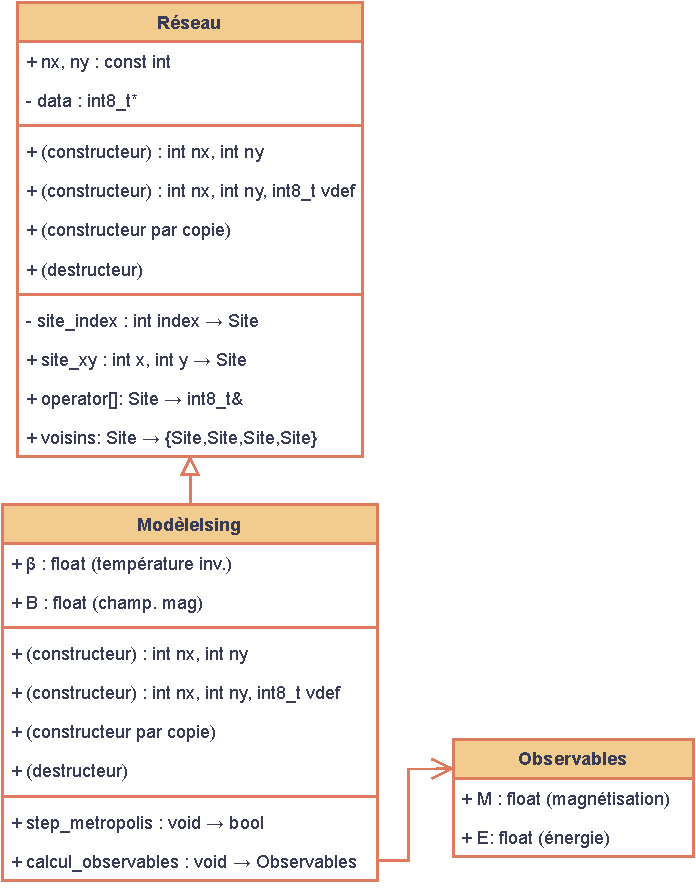
\includegraphics[width=0.55\linewidth]{TD4/diag-classes-ising.pdf}
\caption{Diagramme des classes simplifié.}
\label{fig:diag-classes-ising}
\end{figure}

Le constructeur prenant (\inline{nx},\inline{ny}) comme arguments initialisera le réseau avec des valeurs aléatoires, alors que celui prenant un troisième argument \inline{uint8_t} initialisera un système uniforme, en prenant soin de vérifier que la valeur donnée est bien $\pm 1$. Faites cet exercice de ré-organisation, et testez si votre code fonctionne comme précédemment.

\begin{correction}
Les fichiers de correction (classe \inline{ModèleIsing} et \inline{main()}) sont présents dans le dossier du TD. La classe \inline{Réseau} est inchangée, et le code fonctionne que ce soit pour le réseau carré ou le réseau hexagonal.
\end{correction}

\end{document}
